\apendice{Especificación de Requisitos}
El presente apéndice recoge la documentación técnica detallada sobre la estructura interna y el flujo de ejecución de los componentes que integran el proyecto SugAIr.
\section{Introducción}
Este apéndice tiene como propósito definir y documentar detalladamente los requisitos funcionales y no funcionales que determinan el comportamiento del sistema SugAIr. Para ello, se establece un catálogo de requisitos y se especifican los casos de uso, describiendo las interacciones entre los actores y la propia plataforma. Esta especificación sirve como documento técnico para validar que el \textit{software} construido satisface las necesidades y expectativas detectadas durante la fase de análisis inicial.

\section{Objetivos generales}
El desarrollo de SugAIr persigue proporcionar una herramienta tecnológica privada e inteligente para el apoyo diario a personas con diabetes. Los objetivos generales que guían la especificación de requisitos de este sistema son los siguientes:

\begin{itemize}
    \item \textbf{Centralizar la gestión de la enfermedad:} Aunar en una única plataforma las funciones de educación, predicción y seguimiento de la diabetes mediante el uso de Inteligencia Artificial.
    \item \textbf{Desarrollar un agente especializado:} Proveer un asistente conversacional capaz de contestar preguntas única y exclusivamente sobre diabetes, actuando como un educador diabetológico virtual.
    \item \textbf{Integrar análisis de contexto visual:} Permitir el envío y procesamiento de imágenes (por ejemplo, etiquetas de alimentos) para extraer su valor nutricional, calcular raciones de hidratos de carbono y determinar su velocidad de absorción.
    \item \textbf{Garantizar la privacidad del usuario:} Procesar las interacciones y los datos médicos de forma local, evitando la exposición de información de salud en servidores de terceros.
\end{itemize}

\section{Actores del sistema}
Dado el enfoque de procesamiento local y la ausencia de una arquitectura tradicional con base de datos remota o perfiles de administración, el sistema interactúa de forma exclusiva con un único actor, definido formalmente a continuación:

\begin{itemize}
    \item \textbf{Usuario:} Paciente, familiar o persona interesada que interactúa de forma directa con la interfaz de la aplicación móvil. Es el encargado de formular las consultas de texto, adjuntar las imágenes de las etiquetas nutricionales y recibir la retroalimentación del asistente virtual.
\end{itemize}

\section{Catálogo de requisitos}

Para el desarrollo de SugAIr, se han identificado y clasificado los requisitos en dos grandes grupos: funcionales (aquellos que describen los comportamientos y servicios que el sistema debe proveer) y no funcionales (aquellos que definen atributos de calidad, rendimiento y restricciones del sistema).

\subsection*{Requisitos Funcionales (RF)}
\begin{itemize}
    \item \textbf{RF-01:} El sistema debe permitir al usuario enviar consultas de texto mediante una interfaz de chat.
    \item \textbf{RF-02:} El sistema debe permitir al usuario adjuntar fotografías (ej. etiquetas nutricionales) desde la galería de su dispositivo.
    \item \textbf{RF-03:} El sistema debe recibir, procesar y mostrar en pantalla las respuestas generadas por el motor de IA local.
    \item \textbf{RF-04:} El sistema debe restringir las temáticas de conversación, rechazando o evadiendo aquellas consultas que no estén relacionadas con el ámbito de la diabetes o la nutrición.
\end{itemize}

\subsection*{Requisitos No Funcionales (RNF)}
\begin{itemize}
    \item \textbf{RNF-01 (Privacidad Local):} Todo el procesamiento multimodal y de lenguaje debe ejecutarse en el entorno local del usuario, sin enviar información clínica a servidores externos.
    \item \textbf{RNF-02 (Rendimiento):} El sistema debe ofrecer tiempos de respuesta razonables para un entorno móvil, idealmente devolviendo las respuestas de texto en menos de 15 segundos.
    \item \textbf{RNF-03 (Usabilidad):} La interfaz de usuario debe ser intuitiva, accesible y seguir los estándares de diseño de aplicaciones de mensajería conversacional.
\end{itemize}

\clearpage

\section{Especificación de requisitos}

A continuación, se detallan los Casos de Uso (CU) del sistema, derivados del catálogo de requisitos funcionales. En la figura \ref{fig:casos_uso} se presenta el diagrama general de casos de uso (UML), resumiendo visualmente las interacciones del actor con el sistema.

\begin{figure}[htbp]
    \centering
    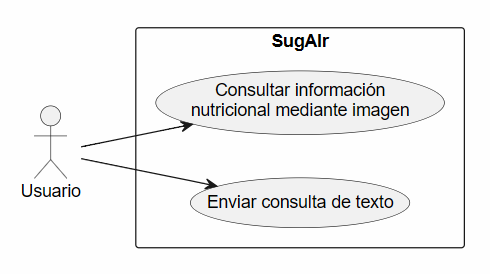
\includegraphics[width=0.8\linewidth]{diagrama de casos de uso.png}
    \caption{Diagrama de casos de uso de SugAIr.}
    \label{fig:casos_uso}
\end{figure}
Cada caso de uso describe una interacción específica entre el Usuario y la aplicación SugAIr, definiendo sus precondiciones, flujo de acciones y posibles excepciones.

% Caso de Uso 1 -> Enviar consulta de texto
\begin{table}[htbp]
    \centering
    \begin{tabularx}{\linewidth}{ p{0.21\columnwidth} p{0.71\columnwidth} }
        \toprule
        \textbf{CU-01}   & \textbf{Enviar consulta de texto}\\
        \toprule
        \textbf{Versión}              & 1.0    \\
        \textbf{Autor}                & Igor Arroyo Ortega \\
        \textbf{Requisitos asociados} & RF-01, RF-03, RF-04 \\
        \textbf{Descripción}          & El usuario formula una pregunta relacionada con la diabetes o nutrición mediante texto y el sistema devuelve una respuesta generada por la IA. \\
        \textbf{Precondición}         & \textbullet~La aplicación debe estar abierta. \newline \textbullet~El servidor backend (Go) y Ollama deben estar en ejecución local. \\
        \textbf{Acciones}             &
        \begin{enumerate}
            \def\labelenumi{\arabic{enumi}.}
            \tightlist
            \item El usuario pulsa sobre la caja de texto en la interfaz del chat.
            \item El usuario escribe su consulta y pulsa el botón de enviar.
            \item La aplicación bloquea el botón de envío y muestra un indicador de carga (\textit{loading}).
            \item El sistema empaqueta la petición en formato JSON y la envía al servidor backend.
            \item El backend consulta al modelo \texttt{llava-diabetes}.
            \item El sistema recibe la respuesta, oculta el indicador de carga y la renderiza en el chat.
        \end{enumerate}\\
        \textbf{Postcondición}        & La conversación queda actualizada en la pantalla con la nueva respuesta del asistente. \\
        \textbf{Excepciones}          & \textbullet~El servidor local está apagado (La app muestra un mensaje de error). \newline \textbullet~Temática no sanitaria (La IA responde recordando sus limitaciones). \\
        \textbf{Importancia}          & Alta \\
        \bottomrule
    \end{tabularx}
    \caption{CU-01: Enviar consulta de texto.}
\end{table}

\vspace{1cm} % Espaciado entre tablas

% Caso de Uso 2 -> Consultar información nutricional mediante imagen
\begin{table}[htbp]
    \centering
    \begin{tabularx}{\linewidth}{ p{0.21\columnwidth} p{0.71\columnwidth} }
        \toprule
        \textbf{CU-02}   & \textbf{Consultar información nutricional mediante imagen}\\
        \toprule
        \textbf{Versión}              & 1.0    \\
        \textbf{Autor}                & Igor Arroyo Ortega \\
        \textbf{Requisitos asociados} & RF-02, RF-03, RF-04 \\
        \textbf{Descripción}          & El usuario adjunta una fotografía (ej. etiqueta de un alimento) para que la IA analice la imagen y extraiga su valor nutricional. \\
        \textbf{Precondición}         & \textbullet~Permisos de galería concedidos en el dispositivo. \newline \textbullet~El servidor backend y Ollama están en ejecución. \\
        \textbf{Acciones}             &
        \begin{enumerate}
            \def\labelenumi{\arabic{enumi}.}
            \tightlist
            \item El usuario pulsa el botón de adjuntar archivo en el chat.
            \item Selecciona una fotografía desde la galería del dispositivo.
            \item La aplicación comprime la imagen y extrae directamente su codificación en formato Base64 puro.
            \item El usuario pulsa enviar (pudiendo añadir texto opcional a la imagen).
            \item El servidor backend recibe la petición y reenvía la cadena Base64 directamente al modelo multimodal.
            \item El sistema recibe y renderiza la respuesta de la IA en la pantalla.
        \end{enumerate}\\
        \textbf{Postcondición}        & La conversación refleja el análisis nutricional devuelto por el asistente basándose en la imagen enviada. \\
        \textbf{Excepciones}          & \textbullet~Permisos de galería denegados por el sistema operativo. \newline \textbullet~Error del servidor (Se captura el estado HTTP y se muestra en pantalla). \\
        \textbf{Importancia}          & Alta \\
        \bottomrule
    \end{tabularx}
    \caption{CU-02: Consultar información nutricional mediante imagen.}
\end{table}
%
\begin{comment}
\apendice{Especificación de Requisitos}

\section{Introducción}

Una muestra de cómo podría ser una tabla de casos de uso:

% Caso de Uso 1 -> Consultar Experimentos.
\begin{table}[p]
	\centering
	\begin{tabularx}{\linewidth}{ p{0.21\columnwidth} p{0.71\columnwidth} }
		\toprule
		\textbf{CU-1}    & \textbf{Ejemplo de caso de uso}\\
		\toprule
		\textbf{Versión}              & 1.0    \\
		\textbf{Autor}                & Alumno \\
		\textbf{Requisitos asociados} & RF-xx, RF-xx \\
		\textbf{Descripción}          & La descripción del CU \\
		\textbf{Precondición}         & Precondiciones (podría haber más de una) \\
		\textbf{Acciones}             &
		\begin{enumerate}
			\def\labelenumi{\arabic{enumi}.}
			\tightlist
			\item Pasos del CU
			\item Pasos del CU (añadir tantos como sean necesarios)
		\end{enumerate}\\
		\textbf{Postcondición}        & Postcondiciones (podría haber más de una) \\
		\textbf{Excepciones}          & Excepciones \\
		\textbf{Importancia}          & Alta o Media o Baja... \\
		\bottomrule
	\end{tabularx}
	\caption{CU-1 Nombre del caso de uso.}
\end{table}

\section{Objetivos generales}

\section{Catálogo de requisitos}

\section{Especificación de requisitos}
\end{comment}

